\PassOptionsToPackage{unicode=true}{hyperref} % options for packages loaded elsewhere
\PassOptionsToPackage{hyphens}{url}
%
\documentclass[
]{article}
\usepackage{lmodern}
\usepackage{amssymb,amsmath}
\usepackage{ifxetex,ifluatex}
\ifnum 0\ifxetex 1\fi\ifluatex 1\fi=0 % if pdftex
  \usepackage[T1]{fontenc}
  \usepackage[utf8]{inputenc}
  \usepackage{textcomp} % provides euro and other symbols
\else % if luatex or xelatex
  \usepackage{unicode-math}
  \defaultfontfeatures{Scale=MatchLowercase}
  \defaultfontfeatures[\rmfamily]{Ligatures=TeX,Scale=1}
\fi
% use upquote if available, for straight quotes in verbatim environments
\IfFileExists{upquote.sty}{\usepackage{upquote}}{}
\IfFileExists{microtype.sty}{% use microtype if available
  \usepackage[]{microtype}
  \UseMicrotypeSet[protrusion]{basicmath} % disable protrusion for tt fonts
}{}
\makeatletter
\@ifundefined{KOMAClassName}{% if non-KOMA class
  \IfFileExists{parskip.sty}{%
    \usepackage{parskip}
  }{% else
    \setlength{\parindent}{0pt}
    \setlength{\parskip}{6pt plus 2pt minus 1pt}}
}{% if KOMA class
  \KOMAoptions{parskip=half}}
\makeatother
\usepackage{xcolor}
\IfFileExists{xurl.sty}{\usepackage{xurl}}{} % add URL line breaks if available
\IfFileExists{bookmark.sty}{\usepackage{bookmark}}{\usepackage{hyperref}}
\hypersetup{
  pdftitle={Stichprobenplanung},
  pdfborder={0 0 0},
  breaklinks=true}
\urlstyle{same}  % don't use monospace font for urls
\usepackage[margin=1in]{geometry}
\usepackage{color}
\usepackage{fancyvrb}
\newcommand{\VerbBar}{|}
\newcommand{\VERB}{\Verb[commandchars=\\\{\}]}
\DefineVerbatimEnvironment{Highlighting}{Verbatim}{commandchars=\\\{\}}
% Add ',fontsize=\small' for more characters per line
\usepackage{framed}
\definecolor{shadecolor}{RGB}{248,248,248}
\newenvironment{Shaded}{\begin{snugshade}}{\end{snugshade}}
\newcommand{\AlertTok}[1]{\textcolor[rgb]{0.94,0.16,0.16}{#1}}
\newcommand{\AnnotationTok}[1]{\textcolor[rgb]{0.56,0.35,0.01}{\textbf{\textit{#1}}}}
\newcommand{\AttributeTok}[1]{\textcolor[rgb]{0.77,0.63,0.00}{#1}}
\newcommand{\BaseNTok}[1]{\textcolor[rgb]{0.00,0.00,0.81}{#1}}
\newcommand{\BuiltInTok}[1]{#1}
\newcommand{\CharTok}[1]{\textcolor[rgb]{0.31,0.60,0.02}{#1}}
\newcommand{\CommentTok}[1]{\textcolor[rgb]{0.56,0.35,0.01}{\textit{#1}}}
\newcommand{\CommentVarTok}[1]{\textcolor[rgb]{0.56,0.35,0.01}{\textbf{\textit{#1}}}}
\newcommand{\ConstantTok}[1]{\textcolor[rgb]{0.00,0.00,0.00}{#1}}
\newcommand{\ControlFlowTok}[1]{\textcolor[rgb]{0.13,0.29,0.53}{\textbf{#1}}}
\newcommand{\DataTypeTok}[1]{\textcolor[rgb]{0.13,0.29,0.53}{#1}}
\newcommand{\DecValTok}[1]{\textcolor[rgb]{0.00,0.00,0.81}{#1}}
\newcommand{\DocumentationTok}[1]{\textcolor[rgb]{0.56,0.35,0.01}{\textbf{\textit{#1}}}}
\newcommand{\ErrorTok}[1]{\textcolor[rgb]{0.64,0.00,0.00}{\textbf{#1}}}
\newcommand{\ExtensionTok}[1]{#1}
\newcommand{\FloatTok}[1]{\textcolor[rgb]{0.00,0.00,0.81}{#1}}
\newcommand{\FunctionTok}[1]{\textcolor[rgb]{0.00,0.00,0.00}{#1}}
\newcommand{\ImportTok}[1]{#1}
\newcommand{\InformationTok}[1]{\textcolor[rgb]{0.56,0.35,0.01}{\textbf{\textit{#1}}}}
\newcommand{\KeywordTok}[1]{\textcolor[rgb]{0.13,0.29,0.53}{\textbf{#1}}}
\newcommand{\NormalTok}[1]{#1}
\newcommand{\OperatorTok}[1]{\textcolor[rgb]{0.81,0.36,0.00}{\textbf{#1}}}
\newcommand{\OtherTok}[1]{\textcolor[rgb]{0.56,0.35,0.01}{#1}}
\newcommand{\PreprocessorTok}[1]{\textcolor[rgb]{0.56,0.35,0.01}{\textit{#1}}}
\newcommand{\RegionMarkerTok}[1]{#1}
\newcommand{\SpecialCharTok}[1]{\textcolor[rgb]{0.00,0.00,0.00}{#1}}
\newcommand{\SpecialStringTok}[1]{\textcolor[rgb]{0.31,0.60,0.02}{#1}}
\newcommand{\StringTok}[1]{\textcolor[rgb]{0.31,0.60,0.02}{#1}}
\newcommand{\VariableTok}[1]{\textcolor[rgb]{0.00,0.00,0.00}{#1}}
\newcommand{\VerbatimStringTok}[1]{\textcolor[rgb]{0.31,0.60,0.02}{#1}}
\newcommand{\WarningTok}[1]{\textcolor[rgb]{0.56,0.35,0.01}{\textbf{\textit{#1}}}}
\usepackage{graphicx,grffile}
\makeatletter
\def\maxwidth{\ifdim\Gin@nat@width>\linewidth\linewidth\else\Gin@nat@width\fi}
\def\maxheight{\ifdim\Gin@nat@height>\textheight\textheight\else\Gin@nat@height\fi}
\makeatother
% Scale images if necessary, so that they will not overflow the page
% margins by default, and it is still possible to overwrite the defaults
% using explicit options in \includegraphics[width, height, ...]{}
\setkeys{Gin}{width=\maxwidth,height=\maxheight,keepaspectratio}
\setlength{\emergencystretch}{3em}  % prevent overfull lines
\providecommand{\tightlist}{%
  \setlength{\itemsep}{0pt}\setlength{\parskip}{0pt}}
\setcounter{secnumdepth}{-2}
% Redefines (sub)paragraphs to behave more like sections
\ifx\paragraph\undefined\else
  \let\oldparagraph\paragraph
  \renewcommand{\paragraph}[1]{\oldparagraph{#1}\mbox{}}
\fi
\ifx\subparagraph\undefined\else
  \let\oldsubparagraph\subparagraph
  \renewcommand{\subparagraph}[1]{\oldsubparagraph{#1}\mbox{}}
\fi

% set default figure placement to htbp
\makeatletter
\def\fps@figure{htbp}
\makeatother

% https://github.com/rstudio/rmarkdown/issues/337
\let\rmarkdownfootnote\footnote%
\def\footnote{\protect\rmarkdownfootnote}

% https://github.com/rstudio/rmarkdown/pull/252
\usepackage{titling}
\setlength{\droptitle}{-2em}

\pretitle{\vspace{\droptitle}\centering\huge}
\posttitle{\par}

\preauthor{\centering\large\emph}
\postauthor{\par}

\predate{\centering\large\emph}
\postdate{\par}

\title{Stichprobenplanung}
\date{}

\begin{document}
\maketitle

\hypertarget{fragestellung}{%
\section{Fragestellung}\label{fragestellung}}

Es ist bekannt, dass etwa 1\% aller Männer rot-blind (protanop) sind. Es
wird vermutet, dass protanope Autofahrer häufiger Auffahrunfälle
verursachen als nicht-protanope Fahrer. Aus diesem Grund wird die
vorerst etwas schwammige Frage formuliert:

\textbf{Sollte protanopen Menschen das Autofahren untersagt werden, da
sie mehr Unfälle verursachen?}

\hypertarget{zielstellung}{%
\section{Zielstellung}\label{zielstellung}}

Wenn protanope Autofahrer genau so fahren würden wie nicht-protanope
Autofahrer, dann müsste der Anteil protanoper Unfallverursacher auch bei
1\% liegen - also so wie in der Gesamtpopulation. (\emph{Anmerkung: Bei
Frauen ist der Anteil deutlich geringer, weswegen sich dieses gesamte
Beispiel nur um männliche Fahrer dreht}) Da keine Daten zum Anteil
protanoper Fahrer in vergangenen Auffahrunfällen erhoben wurden, müsste
Geld investiert werden um dies in Zukunft für eine Stichprobe mit der
Größe \(n\) zu tun. Die Frage ist wie groß \(n\) sein muss um nicht nur
zu einem statistisch signifikanten, sondern auch praktisch relevanten
Ergebnis zu kommen.

\hypertarget{erster-ansatz}{%
\subsection{Erster Ansatz}\label{erster-ansatz}}

Es gilt also zu bestimmen welcher Anteil aller Auffahrunfälle von
protanopen Fahrern verursacht wird und ob dieser erhöht ist. Wir könnten
uns dafür entscheiden ein 95\%-Konfidenzintervall mit einer von uns
gewählten Breite um die jeweils ermittelte Wahrscheinlichkeit zu
berechnen.

Die Formel zur Berechnung solch eines 95\%-Konfidenzintervalls lautet

\[ p ± 1,96 \sqrt{\frac{p(1-p)}{n}}\] wobei \(p\) der
Zielwahrscheinlichkeit entspricht (\emph{Achtung! Hat nichts mit dem
p-Wert zu tun!}). Diese Formel lässt sich auch nach \(n\) umstellen,
sodass wir eine Stichprobenmindestgröße erhalten mit der wir eine
gewünschte Breite des 95\%-Konfidenzintervalls um \(p\) finden:

\[ n = 1,96^2 \frac{p(1-p)}{d^2} \]

wobei \(d\) der halben Breite des angestrebten Konfidenzintervalls
entspricht.

Würden wir nun also \(p=1\%=0,01\) zusammen mit einer angestrebten
halben Breite \(d=0,5\%=0,005\) in die Formel einsetzen, so erhielten
wir eine nötige Stichprobengröße von 1521.2736, aufgerundet also
\(n=1522\):

\begin{Shaded}
\begin{Highlighting}[]
\NormalTok{p <-}\StringTok{ }\FloatTok{0.01}
\NormalTok{d <-}\StringTok{ }\FloatTok{0.005}
\end{Highlighting}
\end{Shaded}

\begin{Shaded}
\begin{Highlighting}[]
\NormalTok{n <-}\StringTok{ }\FloatTok{1.96}\OperatorTok{^}\DecValTok{2} \OperatorTok{*}\StringTok{ }\NormalTok{p}\OperatorTok{*}\NormalTok{(}\DecValTok{1}\OperatorTok{-}\NormalTok{p)}\OperatorTok{/}\NormalTok{d}\OperatorTok{^}\DecValTok{2}
\NormalTok{n}
\end{Highlighting}
\end{Shaded}

\begin{verbatim}
## [1] 1521.274
\end{verbatim}

\begin{Shaded}
\begin{Highlighting}[]
\KeywordTok{ceiling}\NormalTok{(n)}
\end{Highlighting}
\end{Shaded}

\begin{verbatim}
## [1] 1522
\end{verbatim}

Wenn wir also 1522 Auffahrunfälle hinsichtlich der Protanopie des
Unfallverursachers untersuchen würden, würde dies dazu führen, dass bei
\(p=1\%\), alle Wahrscheinlichkeiten \(<0,5\%\) und \(>1,5\%\) nicht
mehr im Konfidenzintervall lägen und somit auch signifikant verschieden
von \(p\) wären.

\begin{Shaded}
\begin{Highlighting}[]
\CommentTok{# Untere Grenze Konfidenzintervall [in %]}
\NormalTok{UKI <-}\StringTok{ }\NormalTok{p }\OperatorTok{-}\StringTok{ }\FloatTok{1.96} \OperatorTok{*}\StringTok{ }\KeywordTok{sqrt}\NormalTok{(p}\OperatorTok{*}\NormalTok{(}\DecValTok{1}\OperatorTok{-}\NormalTok{p)}\OperatorTok{/}\NormalTok{n)}
\NormalTok{UKI}\OperatorTok{*}\DecValTok{100}
\end{Highlighting}
\end{Shaded}

\begin{verbatim}
## [1] 0.5
\end{verbatim}

\begin{Shaded}
\begin{Highlighting}[]
\CommentTok{# Obere Grenze Konfidenzintervall [in %]}
\NormalTok{OKI <-}\StringTok{ }\NormalTok{p }\OperatorTok{+}\StringTok{ }\FloatTok{1.96} \OperatorTok{*}\StringTok{ }\KeywordTok{sqrt}\NormalTok{(p}\OperatorTok{*}\NormalTok{(}\DecValTok{1}\OperatorTok{-}\NormalTok{p)}\OperatorTok{/}\NormalTok{n)}
\NormalTok{OKI}\OperatorTok{*}\DecValTok{100}
\end{Highlighting}
\end{Shaded}

\begin{verbatim}
## [1] 1.5
\end{verbatim}

\begin{Shaded}
\begin{Highlighting}[]
\CommentTok{# Breite Konfidenzintervall [in %]}
\NormalTok{(OKI}\OperatorTok{-}\NormalTok{UKI)}\OperatorTok{*}\DecValTok{100}
\end{Highlighting}
\end{Shaded}

\begin{verbatim}
## [1] 1
\end{verbatim}

Dies wirkt an sich schon wie ein solider Ansatz. Sicherlich sollte das
\(d\) nicht einfach so auf 0,5\% gesetzt werden, sondern stattdessen
eine Abweichung gewählt werden, die sich mit der Wissenschaft und dem
Gesetz vereinbaren lässt. Mit anderen Worten: es muss ein in der Praxis
relevanter Grenzwert gefunden werden, ab dem protanope Fahrer
\emph{bedeutend mehr} Unfälle verursachen als nicht-protanope Fahrer.
Dies ist allerdings kein statistisches Thema und für den Rest dieses
Szenarios werden wir weiterhin mit relevanten Abweichung von 0,5\%
arbeiten. Oder besser gesagt: ab einem Anteil protanoper
Unfallverursacher über 1,5\% sprechen wir davon, dass protanope Fahrer
\emph{bedeutend mehr} Unfälle verursachen als nicht-protanope Fahrer.

\hypertarget{muxe4ngel-des-ersten-ansatzes}{%
\subsubsection{Mängel des ersten
Ansatzes}\label{muxe4ngel-des-ersten-ansatzes}}

Selbst wenn wir uns darauf eingeschossen haben, dass eine Abweichung
\textgreater{} 0,5\% bedeutsam wäre, weist unser Ansatz Mängel auf. So
scheint die Tatsache, dass \(n=1522\) eben nur für \(p=1\%\) gilt, wenig
hilfreich, wenn man länger darüber nachdenkt was zu prüfen ist. Würden
wir in unserer Erhebung herausfinden, dass tatsächlich genau 1\% aller
Unfallverursacher protanop waren, dann wäre ein Blick auf das
Konfidenzintervall völlig hinfällig. Interessant würde es ja erst dann,
wenn der in der Stichprobe gefundene Anteil \(p_1\) eben nicht bei 1\%,
sondern höher liegt. Und hier kommt die Crux: Bei \(n=1522\) und einem
gefundenen Anteil von z.B. \(p_1=1,51\%\) (also mit einer Abweichung von
mehr als 0,5\% !) ergibt sich für das zugehörige 95\%-Konfidenzintervall
wie folgt:

\begin{Shaded}
\begin{Highlighting}[]
\NormalTok{p}\FloatTok{.1}\NormalTok{ <-}\StringTok{ }\FloatTok{0.0151}
\end{Highlighting}
\end{Shaded}

\begin{Shaded}
\begin{Highlighting}[]
\CommentTok{# Untere Grenze Konfidenzintervall [in %]}
\NormalTok{UKI}\FloatTok{.1}\NormalTok{ <-}\StringTok{ }\NormalTok{p}\FloatTok{.1} \OperatorTok{-}\StringTok{ }\FloatTok{1.96} \OperatorTok{*}\StringTok{ }\KeywordTok{sqrt}\NormalTok{(p}\FloatTok{.1}\OperatorTok{*}\NormalTok{(}\DecValTok{1}\OperatorTok{-}\NormalTok{p}\FloatTok{.1}\NormalTok{)}\OperatorTok{/}\NormalTok{n)}
\NormalTok{UKI}\FloatTok{.1}\OperatorTok{*}\DecValTok{100}
\end{Highlighting}
\end{Shaded}

\begin{verbatim}
## [1] 0.8971743
\end{verbatim}

\begin{Shaded}
\begin{Highlighting}[]
\CommentTok{# Obere Grenze Konfidenzintervall [in %]}
\NormalTok{OKI}\FloatTok{.1}\NormalTok{ <-}\StringTok{ }\NormalTok{p}\FloatTok{.1} \OperatorTok{+}\StringTok{ }\FloatTok{1.96} \OperatorTok{*}\StringTok{ }\KeywordTok{sqrt}\NormalTok{(p}\FloatTok{.1}\OperatorTok{*}\NormalTok{(}\DecValTok{1}\OperatorTok{-}\NormalTok{p}\FloatTok{.1}\NormalTok{)}\OperatorTok{/}\NormalTok{n)}
\NormalTok{OKI}\FloatTok{.1}\OperatorTok{*}\DecValTok{100}
\end{Highlighting}
\end{Shaded}

\begin{verbatim}
## [1] 2.122826
\end{verbatim}

\begin{Shaded}
\begin{Highlighting}[]
\CommentTok{# Breite Konfidenzintervall [in %]}
\NormalTok{(OKI}\FloatTok{.1}\OperatorTok{-}\NormalTok{UKI}\FloatTok{.1}\NormalTok{)}\OperatorTok{*}\DecValTok{100}
\end{Highlighting}
\end{Shaded}

\begin{verbatim}
## [1] 1.225651
\end{verbatim}

Wie man sieht, führt ein bestimmtes \(n\) nur für ein bestimmtes \(p\)
zur erwünschten Breite des Konfidenzintervalls. Je weiter sich der
später tatsächlich gefundene Anteil \(p_1\) vom für die
Stichprobenplanung zugrundeliegenden Anteil \(p\) unterscheidet, desto
ungeeigneter ist auch die ursprünglich ermittelte Stichprobengröße
\(n\). In diesem speziellen Fall, liegt der gefundene Anteil
\(p_1=1,51\%\) eigentlich mehr als 0,5\% über den 1\%, jedoch beginnt
sein Konfidenzintervall schon bei 0,897\%, sodass es die 1\% noch mit
einschließt und demnach \(p_1\) nicht signifikant verschieden von 1\%
ist.

\begin{center}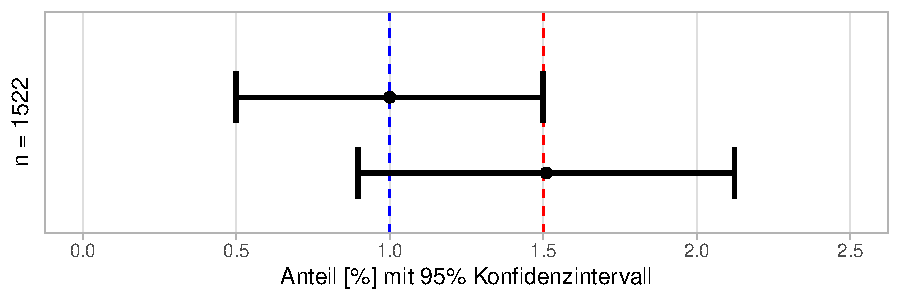
\includegraphics{stat_samplesize_files/figure-latex/unnamed-chunk-11-1} \end{center}

\hypertarget{zweiter-ansatz}{%
\section{Zweiter Ansatz}\label{zweiter-ansatz}}

Zum Vergleich: Die Stichprobengröße, die nötig wäre um ein \(d=0,5\%\)
auch für \(p_1=1,51\%\) einzuhalten, ergibt sich als

\begin{Shaded}
\begin{Highlighting}[]
\NormalTok{n}\FloatTok{.1}\NormalTok{ <-}\StringTok{ }\FloatTok{1.96}\OperatorTok{^}\DecValTok{2} \OperatorTok{*}\StringTok{ }\NormalTok{p}\FloatTok{.1}\OperatorTok{*}\NormalTok{(}\DecValTok{1}\OperatorTok{-}\NormalTok{p}\FloatTok{.1}\NormalTok{)}\OperatorTok{/}\NormalTok{d}\OperatorTok{^}\DecValTok{2}
\KeywordTok{ceiling}\NormalTok{(n}\FloatTok{.1}\NormalTok{)}
\end{Highlighting}
\end{Shaded}

\begin{verbatim}
## [1] 2286
\end{verbatim}

Demnach wird eine größere Stichprobe benötigt, obwohl dieselbe Breite
des Konfidenzintervalls angestrebt wird.

Nun wird also klar, dass es weder mit einem \(n=1522\), noch mit einem
\(n=2286\) getan ist. Das liegt daran, dass wir im Vorfeld keine
Vorstellung davon haben in welchem Bereich sich der tatsächlich
gefundene Anteil protanoper Unfallverursacher \(p_1\) befinden wird.
Klar ist nur, dass es erstrebenswert wäre, dass dessen
Konfidenzintervall den Grenzwert \textbf{nicht} mit einschließt. Da es
hier nur darum geht zu prüfen ob protanope Fahrer eine \emph{erhöhte}
Unfallwahrscheinlichkeit aufweisen, kann man es sogar noch vereinfachen:
So wäre es - unabhängig davon wie groß \(p_1\) ist - erstrebenswert,
dass die untere Grenze von dessen Konfidenzintervall größer als der
Grenzwert ist.

\hypertarget{umdenken}{%
\subsection{Umdenken}\label{umdenken}}

Wenn das gesetzt ist, fällt auf, dass uns auch die angestrebte Breite
des Konfidenzintervalls nur indirekt interessiert. Was wir nämlich zu
Beginn mit der praktisch relevanten Differenz (0,5\%) bzw. dem Grenzwert
(1,5\%) versucht haben, wurde nicht so umgesetzt wie wir es eigentlich
wollten.

Wenn wir wirklich glauben, dass ab einem Wert größer als dem Grenzwert
1,5\%, der Anteil protanoper Unfallverursacher so viel zu hoch ist, dass
sie nicht als gleichwertig sichere Fahrer eingestuft werden sollten,
dann ist unser Zielwert, den wir gerne mit 95\%iger Sicherheit ablehnen
würden ja nicht 1\%, sondern 1,5\% - gegeben dem Fall, dass wir ein
\(p_1\) gefunden haben, dass \textgreater{}1,5\% ist. Was wir also
eigentlich die ganze Zeit wollten ist, dass - unabhängig davon wie groß
das letztendlich gefundene \(p_1\) sein wird - wir eine so große
Stichprobe erheben, dass die untere Grenze des Konfidenzintervalls von
\(p_1\) größer ist als 1,5\%. \emph{(Und nochmal zur Sicherheit: 1,5\%
ergibt sich aus den 1\%, die wir im Normalfall finden würden plus einer
von Experten gewählen praktisch relevanten Erhöhung um 0,5\%)}

\hypertarget{berechnung}{%
\subsection{Berechnung}\label{berechnung}}

Um diese Frage zu beantworten, wollen wir das Ganze für alle \(p_1\)
Werte ab 1,5\% und bis 10,0\% in 0,1\%-Schritten durchrechnen (Infos zur
Nutzung der packages \texttt{data.table} und \texttt{dplyr} gibt's
\href{DatR_MoreAdvanced.html}{hier})

\begin{Shaded}
\begin{Highlighting}[]
\KeywordTok{library}\NormalTok{(data.table)}
\KeywordTok{library}\NormalTok{(dplyr)}

\NormalTok{get.n <-}\StringTok{ }\KeywordTok{data.table}\NormalTok{(}\DataTypeTok{p1.perc =} \KeywordTok{seq}\NormalTok{(}\FloatTok{1.6}\NormalTok{, }\FloatTok{10.0}\NormalTok{, }\FloatTok{0.1}\NormalTok{)) }\OperatorTok\StringTok{ }\CommentTok{# 1,6% - 10,0% in 0,01%-Schritten }
\StringTok{  }\KeywordTok{mutate}\NormalTok{(}\DataTypeTok{p1     =}\NormalTok{ p1.perc}\OperatorTok{/}\DecValTok{100}\NormalTok{,}
         \DataTypeTok{d.perc =}\NormalTok{ p1.perc }\OperatorTok{-}\StringTok{ }\FloatTok{1.5}\NormalTok{, }\CommentTok{# Differenz von p1 zum Grenzwert 1,5%}
         \DataTypeTok{d      =}\NormalTok{  d.perc}\OperatorTok{/}\DecValTok{100}\NormalTok{,}
         \DataTypeTok{n      =} \KeywordTok{ceiling}\NormalTok{((}\FloatTok{1.96}\OperatorTok{^}\DecValTok{2} \OperatorTok{*}\StringTok{ }\NormalTok{p1 }\OperatorTok{*}\StringTok{ }\NormalTok{(}\DecValTok{1}\OperatorTok{-}\NormalTok{p1)) }\OperatorTok{/}\StringTok{ }\NormalTok{d}\OperatorTok{^}\DecValTok{2}\NormalTok{))}
\end{Highlighting}
\end{Shaded}

\begin{Shaded}
\begin{Highlighting}[]
\KeywordTok{head}\NormalTok{(get.n) }\CommentTok{# erste 6 Zeilen}
\end{Highlighting}
\end{Shaded}

\begin{verbatim}
##   p1.perc    p1 d.perc     d     n
## 1     1.6 0.016    0.1 0.001 60483
## 2     1.7 0.017    0.2 0.002 16050
## 3     1.8 0.018    0.3 0.003  7545
## 4     1.9 0.019    0.4 0.004  4476
## 5     2.0 0.020    0.5 0.005  3012
## 6     2.1 0.021    0.6 0.006  2194
\end{verbatim}

\begin{Shaded}
\begin{Highlighting}[]
\KeywordTok{tail}\NormalTok{(get.n) }\CommentTok{# letzte 6 Zeilen}
\end{Highlighting}
\end{Shaded}

\begin{verbatim}
##    p1.perc    p1 d.perc     d  n
## 80     9.5 0.095    8.0 0.080 52
## 81     9.6 0.096    8.1 0.081 51
## 82     9.7 0.097    8.2 0.082 51
## 83     9.8 0.098    8.3 0.083 50
## 84     9.9 0.099    8.4 0.084 49
## 85    10.0 0.100    8.5 0.085 48
\end{verbatim}

\hypertarget{ergebnis}{%
\subsection{Ergebnis}\label{ergebnis}}

So bekommen wir also für all die möglichen \(p_1\) ein entsprechendes
\(n\), mit dem gegeben wäre, dass die untere Grenze des
Konfidenzintervalls um \(p_1\) über 1,5\% liegt. In der ersten Zeile
sehen wir, dass bei \(p_1=1,6\%\) gut 60.000 Unfallversursacher
untersucht werden müssten um die relativ kleine Abweichung von 0.1\%
über dem Grenzwert als statistisch abgesichert einstufen zu können. Es
ergibt Sinn, dass bei \(p_1=10,0%
\) (letzte Zeile) nur 48 Unfallverursacher untersucht werden müssten um
die große Abweichung von 8,5\% als statistische signifikant zu
identifzieren.

Mit diesen Berechnungen kann nun mit Experten darüber disktutiert werden
was für eine Abweichung zu erwarten ist und wie groß die Stichprobe
gewählt werden sollte.

Dies ist bereits das von uns angestrebte Ergebnis, wir wollen die
Ergebnistabelle aber noch mit weiteren nützlichen Informationen füllen:

\begin{Shaded}
\begin{Highlighting}[]
\NormalTok{get.n <-}\StringTok{ }\NormalTok{get.n }\OperatorTok
\StringTok{  }\KeywordTok{mutate}\NormalTok{(}\DataTypeTok{n.prot =} \KeywordTok{ceiling}\NormalTok{(n}\OperatorTok{*}\NormalTok{p1),                   }\CommentTok{# Absolute Anzahl protanoper Fahrer}
         \DataTypeTok{U.KI   =}\NormalTok{ p1 }\OperatorTok{-}\StringTok{ }\FloatTok{1.96} \OperatorTok{*}\StringTok{ }\KeywordTok{sqrt}\NormalTok{( p1}\OperatorTok{*}\NormalTok{(}\DecValTok{1}\OperatorTok{-}\NormalTok{p1)}\OperatorTok{/}\NormalTok{n ), }\CommentTok{# Untere Grenze}
         \DataTypeTok{O.KI   =}\NormalTok{ p1 }\OperatorTok{+}\StringTok{ }\FloatTok{1.96} \OperatorTok{*}\StringTok{ }\KeywordTok{sqrt}\NormalTok{( p1}\OperatorTok{*}\NormalTok{(}\DecValTok{1}\OperatorTok{-}\NormalTok{p1)}\OperatorTok{/}\NormalTok{n ), }\CommentTok{# Obere  Grenze}
         \DataTypeTok{RR     =} \KeywordTok{round}\NormalTok{(p1}\OperatorTok{/}\NormalTok{(}\FloatTok{1.0}\OperatorTok{/}\DecValTok{100}\NormalTok{),}\DecValTok{1}\NormalTok{)) }\CommentTok{# Relatives Risiko (annäherungsweise)}

\KeywordTok{head}\NormalTok{(get.n) }\CommentTok{# Erste 6 Zeilen}
\end{Highlighting}
\end{Shaded}

\begin{verbatim}
##   p1.perc    p1 d.perc     d     n n.prot       U.KI       O.KI  RR
## 1     1.6 0.016    0.1 0.001 60483    968 0.01500001 0.01699999 1.6
## 2     1.7 0.017    0.2 0.002 16050    273 0.01500005 0.01899995 1.7
## 3     1.8 0.018    0.3 0.003  7545    136 0.01500002 0.02099998 1.8
## 4     1.9 0.019    0.4 0.004  4476     86 0.01500035 0.02299965 1.9
## 5     2.0 0.020    0.5 0.005  3012     61 0.01500015 0.02499985 2.0
## 6     2.1 0.021    0.6 0.006  2194     47 0.01500017 0.02699983 2.1
\end{verbatim}

\begin{Shaded}
\begin{Highlighting}[]
\KeywordTok{tail}\NormalTok{(get.n) }\CommentTok{# Letzte 6 Zeilen}
\end{Highlighting}
\end{Shaded}

\begin{verbatim}
##    p1.perc    p1 d.perc     d  n n.prot       U.KI      O.KI   RR
## 80     9.5 0.095    8.0 0.080 52      5 0.01530327 0.1746967  9.5
## 81     9.6 0.096    8.1 0.081 51      5 0.01514799 0.1768520  9.6
## 82     9.7 0.097    8.2 0.082 51      5 0.01577294 0.1782271  9.7
## 83     9.8 0.098    8.3 0.083 50      5 0.01558858 0.1804114  9.8
## 84     9.9 0.099    8.4 0.084 49      5 0.01537464 0.1826254  9.9
## 85    10.0 0.100    8.5 0.085 48      5 0.01512951 0.1848705 10.0
\end{verbatim}

Die Spalte \texttt{n.prot} gibt die Anzahl protanoper Fahrer an, die in
der Stichprobe mit Größe \(n\) dem Anteil \(p_1\) entspricht. Bezogen
auf die erste Zeile bedeutet das: wenn mindestens 968 der 60.483
Unfallverursacher protanop wären, dann entspräche dies einem \(p_1\) von
mindestens 1,6\% und dessen untere Grenze des Konfidenzintervalls würde
die 1,5\% nicht mehr miteinschließen (siehe auch Spalte \texttt{U.KI}).

Das Relative Risiko (Risk Ratio), auf das hier nur sehr kurz eingegangen
werden soll (mehr Infos z.B.
\href{https://www.wikiwand.com/de/Relatives_Risiko}{hier}), wurde hier
zusätzlich und nur annäherungsweise geschätzt. Die Annäherung rührt
daher, dass man für dieses Maß auch den Anteil protanoper Männer an
Autofahrern \emph{ohne} Unfall benötigt. Dieser wurde zur Berechnung
einfach auf die 1\% gesetzt, was hier übrigens dazu führt, dass
\(RR=p_1\). Ein relatives Risiko von 2 würde bedeuten, dass das Risiko
einen Unfall zu verursachen unter protanopen Autofahrern 2-mal so hoch
ist wie unter nicht-protanopen Autofahrern.

\hypertarget{graphische-darstellung}{%
\subsection{Graphische Darstellung}\label{graphische-darstellung}}

Diese Ergebnisse sollen schließlich noch grafisch dargestellt werden:

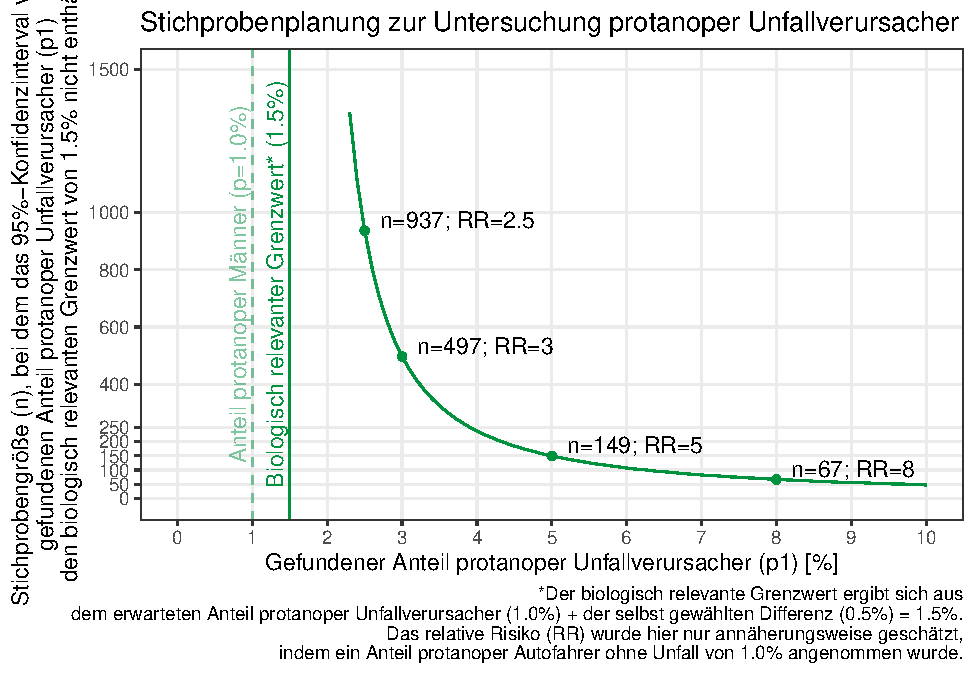
\includegraphics{stat_samplesize_files/figure-latex/unnamed-chunk-17-1.pdf}

Und hier eine detaillierte Erklärung zur Erstellung des Plots mit den
packages \texttt{ggplot2} und \texttt{ggrepel}. Bevor wir die Ergebnisse
plotten, erstellen wir aus ihnen einen Teildatensatz mit einer Hand voll
markanter Werte, die wir im Plot extra hervorheben wollen:

\begin{Shaded}
\begin{Highlighting}[]
\NormalTok{label.tab <-}\StringTok{ }\NormalTok{get.n }\OperatorTok
\StringTok{  }\KeywordTok{filter}\NormalTok{(p1.perc }\OperatorTok\StringTok{ }\KeywordTok{c}\NormalTok{(}\FloatTok{2.5}\NormalTok{, }\DecValTok{3}\NormalTok{, }\DecValTok{5}\NormalTok{, }\DecValTok{8}\NormalTok{)) }\OperatorTok\StringTok{ }\CommentTok{# Auswahl dieser 4 Werte}
\StringTok{  }\KeywordTok{select}\NormalTok{(n, p1.perc, RR) }\OperatorTok\StringTok{ }\CommentTok{# Behalte nur relevante Spalten}
\StringTok{  }\KeywordTok{mutate}\NormalTok{(}\DataTypeTok{labeltext =} \KeywordTok{paste0}\NormalTok{(}\StringTok{"n="}\NormalTok{,n,}\StringTok{"; RR="}\NormalTok{, RR)) }\CommentTok{# Erstellen eines Labels für jeden Wert}

\NormalTok{label.tab}
\end{Highlighting}
\end{Shaded}

\begin{verbatim}
##     n p1.perc  RR     labeltext
## 1 937     2.5 2.5 n=937; RR=2.5
## 2 497     3.0 3.0   n=497; RR=3
## 3 149     5.0 5.0   n=149; RR=5
## 4  67     8.0 8.0    n=67; RR=8
\end{verbatim}

Der Plot wurde mit folgendem Code erstellt:

\begin{Shaded}
\begin{Highlighting}[]
\KeywordTok{library}\NormalTok{(ggplot2)}
\KeywordTok{library}\NormalTok{(ggrepel) }\CommentTok{# package um einzelne Datenpunkte in einem Plot mit einem Label zu versehen}

\KeywordTok{ggplot}\NormalTok{() }\OperatorTok{+}\StringTok{ }
\StringTok{  }\CommentTok{# Vertikale Linie bei 1.0%}
\StringTok{  }\KeywordTok{geom_vline}\NormalTok{(}\DataTypeTok{xintercept=}\FloatTok{1.0}\NormalTok{, }\DataTypeTok{linetype=}\StringTok{"dashed"}\NormalTok{, }\DataTypeTok{color=}\StringTok{"#00923F"}\NormalTok{, }\DataTypeTok{alpha=}\FloatTok{0.5}\NormalTok{) }\OperatorTok{+}\StringTok{ }
\StringTok{  }\CommentTok{# Label neben der vertikalen Linie (bei 0.8%)}
\StringTok{  }\KeywordTok{geom_text}\NormalTok{(}\KeywordTok{aes}\NormalTok{(}\DataTypeTok{x=}\FloatTok{0.8}\NormalTok{, }\DataTypeTok{y=}\DecValTok{750}\NormalTok{, }\DataTypeTok{label=}\KeywordTok{paste0}\NormalTok{(}\StringTok{"Anteil protanoper Männer (p=1.0%)"}\NormalTok{)), }
            \DataTypeTok{colour=}\StringTok{"#00923F"}\NormalTok{, }\DataTypeTok{angle=}\DecValTok{90}\NormalTok{, }\DataTypeTok{alpha=}\FloatTok{0.5}\NormalTok{) }\OperatorTok{+}\StringTok{ }
\StringTok{  }\CommentTok{# Vertikale Linie bei 1.5%}
\StringTok{  }\KeywordTok{geom_vline}\NormalTok{(}\DataTypeTok{xintercept=}\FloatTok{1.5}\NormalTok{, }\DataTypeTok{linetype=}\StringTok{"solid"}\NormalTok{, }\DataTypeTok{color=}\StringTok{"#00923F"}\NormalTok{) }\OperatorTok{+}\StringTok{ }
\StringTok{  }\CommentTok{# Label neben der vertikalen Linie (bei 1.3%)}
\StringTok{  }\KeywordTok{geom_text}\NormalTok{(}\KeywordTok{aes}\NormalTok{(}\DataTypeTok{x=}\FloatTok{1.3}\NormalTok{, }\DataTypeTok{y=}\DecValTok{750}\NormalTok{, }\DataTypeTok{label=}\KeywordTok{paste0}\NormalTok{(}\StringTok{"Biologisch relevanter Grenzwert* (1.5%)"}\NormalTok{)), }
            \DataTypeTok{colour=}\StringTok{"#00923F"}\NormalTok{, }\DataTypeTok{angle=}\DecValTok{90}\NormalTok{) }\OperatorTok{+}\StringTok{ }
\StringTok{  }\CommentTok{# Linie für alle ermittelten n (data=get.n)}
\StringTok{  }\KeywordTok{geom_line}\NormalTok{(}\DataTypeTok{data=}\NormalTok{get.n, }\KeywordTok{aes}\NormalTok{(}\DataTypeTok{y=}\NormalTok{n, }\DataTypeTok{x=}\NormalTok{p1.perc), }\DataTypeTok{color=}\StringTok{"#00923F"}\NormalTok{) }\OperatorTok{+}\StringTok{ }
\StringTok{  }\CommentTok{# Punkte nur für ausgewählte n (data=label.tab)}
\StringTok{  }\KeywordTok{geom_point}\NormalTok{(}\DataTypeTok{data=}\NormalTok{label.tab, }\KeywordTok{aes}\NormalTok{(}\DataTypeTok{y=}\NormalTok{n, }\DataTypeTok{x=}\NormalTok{p1.perc), }\DataTypeTok{color=}\StringTok{"#00923F"}\NormalTok{) }\OperatorTok{+}\StringTok{ }
\StringTok{  }\CommentTok{# Punkte-Label nur für ausgewählte n (data=label.tab)}
\StringTok{  }\KeywordTok{geom_text_repel}\NormalTok{(}\DataTypeTok{data=}\NormalTok{label.tab, }\KeywordTok{aes}\NormalTok{(}\DataTypeTok{y=}\NormalTok{n, }\DataTypeTok{x=}\NormalTok{p1.perc, }\DataTypeTok{label=}\NormalTok{labeltext), }
                  \DataTypeTok{nudge_x =} \FloatTok{0.2}\NormalTok{, }\DataTypeTok{nudge_y =} \DecValTok{10}\NormalTok{, }\DataTypeTok{vjust=}\DecValTok{0}\NormalTok{, }\DataTypeTok{hjust=}\DecValTok{0}\NormalTok{) }\OperatorTok{+}\StringTok{ }
\StringTok{  }\CommentTok{# Formatiere x-Achse}
\StringTok{  }\KeywordTok{scale_x_continuous}\NormalTok{(}\DataTypeTok{name =} \KeywordTok{paste0}\NormalTok{(}\StringTok{"Gefundener Anteil protanoper Unfallverursacher (p1) [%]"}\NormalTok{), }
                     \DataTypeTok{breaks =} \KeywordTok{seq}\NormalTok{(}\DecValTok{0}\NormalTok{,}\DecValTok{10}\NormalTok{,}\DecValTok{1}\NormalTok{), }\DataTypeTok{limits =} \KeywordTok{c}\NormalTok{(}\DecValTok{0}\NormalTok{,}\DecValTok{10}\NormalTok{)) }\OperatorTok{+}\StringTok{ }
\StringTok{  }\CommentTok{# Formatiere y-Achse}
\StringTok{  }\KeywordTok{scale_y_continuous}\NormalTok{(}\DataTypeTok{name =} \KeywordTok{paste0}\NormalTok{(}\StringTok{"Stichprobengröße (n), bei dem das 95%-Konfidenzinterval vom}\CharTok{\textbackslash{}n}\StringTok{ gefundenen Anteil protanoper Unfallverursacher (p1) }\CharTok{\textbackslash{}n}\StringTok{ den biologisch relevanten Grenzwert von 1.5% nicht enthält"}\NormalTok{), }\DataTypeTok{breaks =} \KeywordTok{c}\NormalTok{(}\DecValTok{0}\NormalTok{,}\DecValTok{50}\NormalTok{,}\DecValTok{100}\NormalTok{,}\DecValTok{150}\NormalTok{,}\DecValTok{200}\NormalTok{,}\DecValTok{250}\NormalTok{,}\DecValTok{400}\NormalTok{,}\DecValTok{600}\NormalTok{,}\DecValTok{800}\NormalTok{,}\DecValTok{1000}\NormalTok{, }\DecValTok{1500}\NormalTok{), }\DataTypeTok{limits =} \KeywordTok{c}\NormalTok{(}\DecValTok{0}\NormalTok{,}\DecValTok{1500}\NormalTok{)) }\OperatorTok{+}\StringTok{ }
\StringTok{  }\CommentTok{# Title und Anmerkung unterm Plot}
\StringTok{  }\KeywordTok{labs}\NormalTok{(}\DataTypeTok{title    =} \StringTok{"Stichprobenplanung zur Untersuchung protanoper Unfallverursacher"}\NormalTok{,}
       \DataTypeTok{caption  =} \StringTok{"*Der biologisch relevante Grenzwert ergibt sich aus}\CharTok{\textbackslash{}n}\StringTok{ dem erwarteten Anteil protanoper Unfallverursacher (1.0%) + der selbst gewählten Differenz (0.5%) = 1.5%.}\CharTok{\textbackslash{}n}\StringTok{ Das relative Risiko (RR) wurde hier nur annäherungsweise geschätzt,}\CharTok{\textbackslash{}n}\StringTok{ indem ein Anteil protanoper Autofahrer ohne Unfall von 1.0% angenommen wurde."}\NormalTok{) }\OperatorTok{+}\StringTok{ }
\StringTok{  }\CommentTok{# Formatvorlage (Hintergrundfarbe usw.)}
\StringTok{  }\KeywordTok{theme_bw}\NormalTok{() }\OperatorTok{+}\StringTok{ }
\StringTok{  }\CommentTok{# Zeige nur die Hilfslinien an, die auch Werte an den Achsen haben}
\StringTok{  }\KeywordTok{theme}\NormalTok{(}\DataTypeTok{panel.grid.minor =} \KeywordTok{element_blank}\NormalTok{())}
\end{Highlighting}
\end{Shaded}

\end{document}
